%% Sección principal: Problemas de Factibilidad y Optimización
\section{Problemas de Factibilidad y Optimización}\label{sec:main_fact_opt}

Los problemas de factibilidad y optimización son pilares fundamentales en la modelización y resolución de una
vasta gama de desafíos en la ingeniería, las ciencias computacionales, la economía y la investigación operativa.
Un problema de optimización, en su forma más general, busca seleccionar la ``mejor'' alternativa de un conjunto
de opciones posibles, sujeta a ciertas limitaciones~\cite[p.~1]{BoydVandenberghe2004},~\cite[p.~4]{BoydVandenbergheSlides2023}. Por otro lado, un problema de factibilidad se centra en determinar
si existe al menos una solución que satisfaga un conjunto dado de restricciones, sin considerar necesariamente
un criterio de optimalidad~\cite[p.~130]{BoydVandenberghe2004},~\cite[p.~1]{Sidford2020}. Esta sección definirá
formalmente ambos tipos de problemas, explorará su interrelación y cómo los problemas de factibilidad pueden
ser vistos como un subconjunto de los problemas de optimización.

%% Subsección: Problemas de Optimización
\subsection{Problemas de Optimización}\label{sec:opt_problems}

Un \textbf{problema de optimización matemática}\footnote{\textbf{Problema de optimización matemática:}
También conocido como problema de programación matemática. Consiste en seleccionar la mejor solución
(según algún criterio cuantificado por la función objetivo) de un conjunto de alternativas factibles
(definidas por las restricciones)~\cite[p.~1]{BoydVandenberghe2004}.} se puede expresar en su forma
estándar como~\cite[p.~127]{BoydVandenberghe2004},~\cite[p.~89]{BoydVandenbergheSlides2023}:

\begin{align}
  \text{minimizar} \quad & f_0(x) \\
  \text{sujeto a} \quad & g_i(x) \leq 0, \quad i = 1, \dots, m \\
                      & h_j(x) = 0,    \quad j = 1, \dots, p
\end{align}

donde:
\begin{itemize}
    \item $x \in \mathbb{R}^n$ es el \textbf{vector de variables de optimización}\footnote{\textbf{Vector de
          variables de optimización:} El vector $x = (x_1, \dots, x_n)$ contiene las cantidades que se pueden
          elegir o variar para encontrar la solución óptima. La dimensión $n$ es el número de variables escalares~\cite[p.~1]{BoydVandenberghe2004}.} (o variables de decisión).
    \item $f_0: \mathbb{R}^n \to \mathbb{R}$ es la \textbf{función objetivo}\footnote{\textbf{Función objetivo:}
          La función $f_0: \mathbb{R}^n \to \mathbb{R}$ cuyo valor se busca minimizar (o maximizar). Cuantifica
          el rendimiento, costo, utilidad o mérito asociado a una elección particular de las variables de optimización~\cite[p.~1]{BoydVandenberghe2004}.}, la cual se desea minimizar (o maximizar, lo que es equivalente a
          minimizar $-f_0$).
    \item $g_i: \mathbb{R}^n \to \mathbb{R}$, para $i = 1, \dots, m$, son las \textbf{funciones de restricción
          de desigualdad}.
    \item $h_j: \mathbb{R}^n \to \mathbb{R}$, para $j = 1, \dots, p$, son las \textbf{funciones de restricción
          de igualdad} (usualmente deben ser afines en problemas de optimización convexa).
\end{itemize}

El conjunto $\mathcal{D} = \left(\bigcap_{i=0}^m \text{dom}(f_i)\right) \cap \left(\bigcap_{j=1}^p \text{dom}(h_j)\right)$
es el \textbf{dominio} del problema. Un punto $x \in \mathcal{D}$ es \textbf{factible} si satisface todas las
restricciones. El conjunto de todos los puntos factibles se denomina \textbf{conjunto factible} o \textbf{región factible}~\cite[p.~128]{BoydVandenberghe2004},~\cite[p.~90]{BoydVandenbergheSlides2023}. Si el conjunto factible es vacío,
el problema es \textbf{infactible}. El valor $p^* = \inf\{f_0(x) \mid x \text{ es factible}\}$ es el \textbf{valor óptimo}.
Si existe un $x^*$ tal que $f_0(x^*) = p^*$, entonces $x^*$ es un \textbf{punto óptimo} (global)~\cite[p.~128]{BoydVandenberghe2004},~\cite[p.~90]{BoydVandenbergheSlides2023}.

\begin{figure}
    \centering
    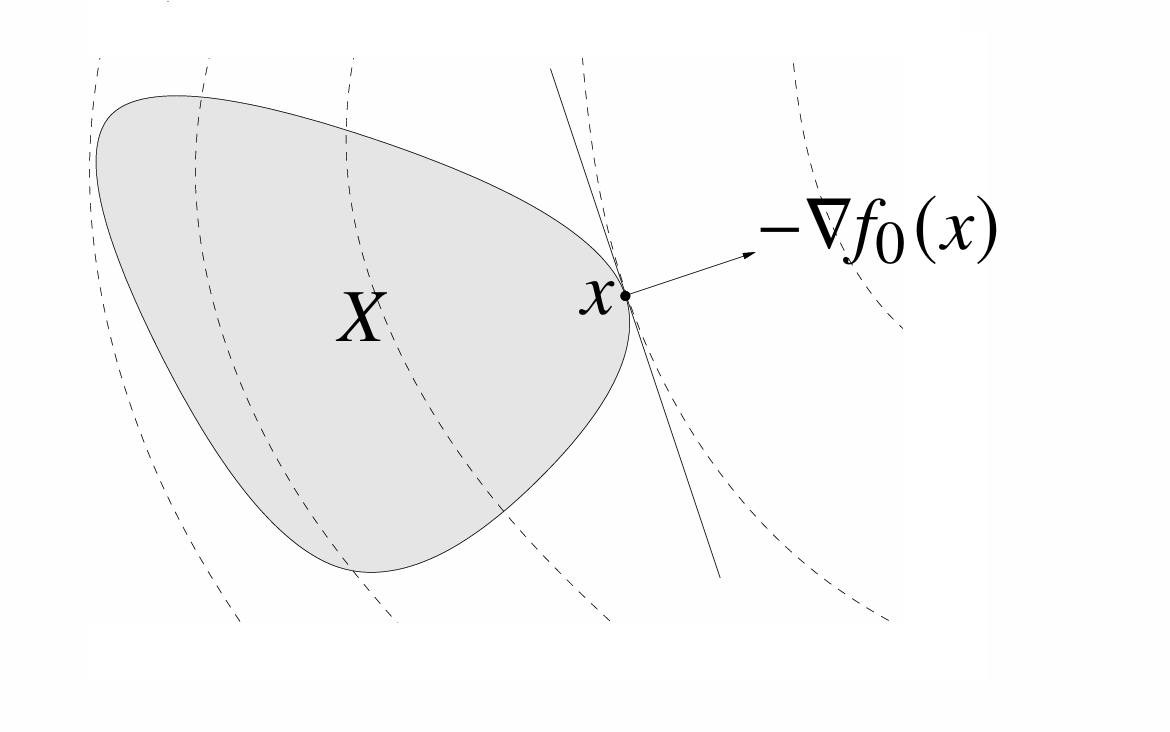
\includegraphics[width=\linewidth]{img//marcoTeorico/optimizacion_fig1.png}
    \caption{Gráfica 2D que muestre contornos de una función objetivo $f_0(x)$,
              una región factible sombreada definida por restricciones, y el punto óptimo $x^*$.}%
    \label{fig:enter-label}
\end{figure}

Los problemas de optimización se clasifican según la naturaleza de sus funciones objetivo y de restricción.
Los \textbf{problemas de programación lineal (LP)}\footnote{\textbf{Programación Lineal (LP):} Un problema de
optimización donde tanto la función objetivo $f_0$ como todas las funciones de restricción $f_i$ y $h_j$ son afines
(lineales más una constante)~\cite[p.~4]{BoydVandenberghe2004},~\cite[p.~101]{BoydVandenbergheSlides2023}.} tienen
funciones objetivo y de restricción afines~\cite[p.~4]{BoydVandenberghe2004},~\cite[p.~101]{BoydVandenbergheSlides2023}.
Los \textbf{problemas de programación cuadrática (QP)}\footnote{\textbf{Programación Cuadrática (QP):} Un problema de
optimización donde la función objetivo $f_0$ es cuadrática (y usualmente convexa para garantizar tratabilidad) y las
funciones de restricción $f_i$ y $h_j$ son afines~\cite[p.~152]{BoydVandenberghe2004},~\cite[p.~105]{BoydVandenbergheSlides2023}.} implican minimizar una función objetivo cuadrática convexa sobre un
poliedro (definido por restricciones afines)~\cite[p.~152]{BoydVandenberghe2004},~\cite[p.~105]{BoydVandenbergheSlides2023}.

Un caso particularmente importante es la \textbf{optimización convexa}, donde la función objetivo $f_0$ y las funciones
de restricción de desigualdad $f_1, \dots, f_m$ son funciones convexas\footnote{\textbf{Función convexa:} Una función
$f: \mathbb{R}^n \to \mathbb{R}$ es convexa si su dominio $\text{dom}(f)$ es un conjunto convexo y para todo $x, y \in \text{dom}(f)$
y todo $\theta$ con $0 \leq \theta \leq 1$, se cumple la desigualdad de Jensen: $f(\theta x + (1 - \theta)y) \leq \theta f(x) + (1 - \theta)f(y)$~\cite[p.~67]{BoydVandenberghe2004},~\cite[p.~46]{BoydVandenbergheSlides2023}. Geométricamente, el segmento de línea que
une dos puntos cualesquiera $(x, f(x))$ e $(y, f(y))$ en la gráfica de la función se encuentra por encima o sobre la gráfica de $f$.},
y las funciones de restricción de igualdad $h_j$ son afines (es decir, de la forma $Ax = b$)~\cite[p.~7]{BoydVandenberghe2004},~\cite[pp.~13, 95]{BoydVandenbergheSlides2023}. La optimización convexa es fundamental
porque, a diferencia de los problemas de optimización no lineal generales, cualquier óptimo local es también un óptimo global,
y existen algoritmos eficientes y confiables para resolverlos~\cite[pp.~8-9]{BoydVandenberghe2004},~\cite[pp.~10-11, 97]{BoydVandenbergheSlides2023}. Otros tipos relevantes incluyen la optimización no lineal (general),
la optimización discreta (o entera), la optimización estocástica y la optimización robusta~\cite[pp.~9-10]{BoydVandenberghe2004}.

Las aplicaciones típicas de la optimización matemática son vastas e incluyen el diseño de ingeniería (e.g., diseño de
dispositivos, estructuras), el análisis y ajuste de datos (e.g., regresión, clasificación), la economía (e.g., modelos
de equilibrio), y la gestión y finanzas (e.g., optimización de carteras, planificación de producción)~\cite[pp.~2-3]{BoydVandenberghe2004}. Por ejemplo, en el ajuste de datos, $x$ puede representar los parámetros de un
modelo y $f_0(x)$ una medida del error de predicción, a menudo con un término de regularización para penalizar la
complejidad del modelo y evitar el sobreajuste~\cite[p.~6]{BoydVandenbergheSlides2023}. En la optimización de carteras,
$x$ podría representar las asignaciones de inversión en diferentes activos, las restricciones podrían incluir el presupuesto
total y los requisitos mínimos de retorno, y $f_0(x)$ podría ser el riesgo (e.g., la varianza del retorno) que se busca
minimizar~\cite[p.~2]{BoydVandenberghe2004}.

%% Subsección: Problemas de Factibilidad
\subsection{Problemas de Factibilidad}\label{sec:feas_problems}

Un \textbf{problema de factibilidad} consiste simplemente en encontrar un punto $x$ que satisfaga un conjunto de
restricciones, sin una función objetivo explícita que optimizar~\cite[p.~130]{BoydVandenberghe2004},~\cite[p.~1]{Sidford2020}:

\begin{align}
  \text{encontrar} \quad & x \\
  \text{sujeto a} \quad  & g_i(x) \leq 0, \quad i = 1, \dots, m \\
                       & h_j(x) = 0,    \quad j = 1, \dots, p
\end{align}

La pregunta fundamental es si el conjunto factible (el conjunto de todos los $x$ que satisfacen las restricciones)
es no vacío. Si existe al menos un $x$ que cumple todas las restricciones, el problema es \textbf{factible} y cualquier
$x$ de este tipo es una solución. De lo contrario, si el conjunto factible es vacío, el problema es \textbf{infactible}~\cite[p.~129]{BoydVandenberghe2004},~\cite[p.~94]{BoydVandenbergheSlides2023}.

Sidford~\cite[p.~2]{Sidford2020} presenta una definición más algorítmica para el problema de factibilidad, particularmente
en el contexto de los \textbf{métodos de planos cortantes}\footnote{\textbf{Métodos de planos cortantes
(\textit{Cutting Plane Methods}):} Una clase de algoritmos utilizados para resolver problemas de optimización (a menudo
convexos o problemas de optimización entera). Funcionan refinando iterativamente una aproximación poliédrica del conjunto
factible o del epígrafe de la función objetivo, añadiendo ``planos cortantes'' (restricciones de hiperplanos) que eliminan
regiones del espacio de búsqueda que se garantiza que no contienen la solución óptima, sin eliminar la propia solución óptima~\cite[p.~1]{Sidford2020}.}. Para $0 < r < R$ y $n \geq 1$, el problema de factibilidad $(r, R, n)$ se define de la
siguiente manera: se dispone de un \textbf{oráculo de separación}\footnote{\textbf{Oráculo de separación
(\textit{Separation Oracle}):} Para un conjunto convexo $C \subseteq \mathbb{R}^n$, un oráculo de separación es un
procedimiento que, dado un punto $x \in \mathbb{R}^n$, o bien determina que $x \in C$, o bien devuelve un hiperplano
que separa $x$ de $C$. Es decir, encuentra un vector $a \in \mathbb{R}^n$ y un escalar $b \in \mathbb{R}$ tales que
$a^T x > b$ mientras que $a^T z \leq b$ para todo $z \in C$~\cite[p.~1]{Sidford2020}. En el contexto de la definición
de Sidford, $g_x$ es el vector normal a tal hiperplano separador.} que, al ser consultado con un punto $x \in B_\infty(R)$
(una bola en la norma infinito de radio $R$ centrada en el origen), produce un vector $g_x \in \mathbb{R}^n$.
El objetivo es uno de los siguientes:

\begin{enumerate}
    \item Encontrar algún $x \in B_\infty(R)$ tal que $g_x = 0$ (este $x$ se considera un ``punto bueno'' que satisface
          la condición de factibilidad implícita del oráculo).
    \item Encontrar un conjunto de puntos $x_1, \dots, x_k \in B_\infty(R)$ tales que la región
          $S = B_\infty(R) \cap_{i \in [k]} \text{half}(g_{x_i}, g_{x_i}^T x_i)$ (la intersección de la bola inicial
          con los semiespacios definidos por los vectores $g_{x_i}$) no contenga ninguna bola de radio $r$.
\end{enumerate}

\begin{figure}
    \centering
    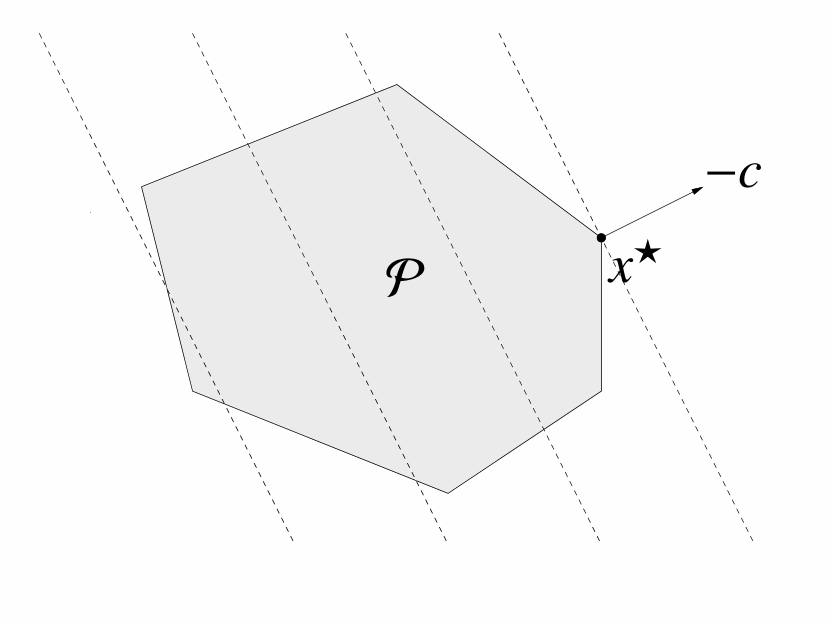
\includegraphics[width=0.75\linewidth]{img//marcoTeorico/optimizacion_fig2.png}
    \caption{Representación bidimensional de un conjunto de restricciones lineales (líneas rectas) que definen una región poliédrica sombreada correspondiente al conjunto factible de un problema de programación lineal (LP). Se ilustran además los contornos paralelos de la función objetivo lineal y la dirección de optimización. Adaptada de~\cite[p.~101]{BoydVandenbergheSlides2023}}%
    \label{fig:optimization2}
\end{figure}

Este enfoque es fundamental para algoritmos que iterativamente refinan una región de búsqueda. Utilizan los hiperplanos
generados por el oráculo para ``cortar'' o eliminar porciones del espacio de búsqueda que se sabe que no contienen
soluciones factibles, hasta que se encuentra una solución o se demuestra que la región de soluciones ``buenas'' (si existen)
es demasiado pequeña para ser relevante (de radio menor que $r$)~\cite[pp.~1, 5]{Sidford2020}.

Los problemas de factibilidad son cruciales en diversas áreas. Por ejemplo, en la minimización de funciones, muchos
algoritmos de optimización, especialmente los métodos de punto interior, requieren un punto inicial factible (o incluso
estrictamente factible) para comenzar~\cite[p.~579]{BoydVandenberghe2004},~\cite[p.~372]{BoydVandenbergheSlides2023}.
Determinar la existencia de tal punto es en sí mismo un problema de factibilidad. También surgen intrínsecamente en el
estudio de oráculos de separación para conjuntos y funciones convexas, que son componentes básicos de muchos algoritmos
de optimización eficientes~\cite[p.~1]{Sidford2020}.

%% Subsección: Relación y Contención
\subsection{Relación y Contención}\label{sec:relation_containment}

La relación entre los problemas de factibilidad y optimización es intrínseca y fundamental. Todo problema de optimización
inherentemente contiene un problema de factibilidad subyacente: antes de poder encontrar la ``mejor'' solución (óptima),
primero se debe determinar si existe \textit{alguna} solución que satisfaga todas las restricciones impuestas. Si el
conjunto factible es vacío, el problema de optimización es infactible y, por lo tanto, no tiene solución~\cite[p.~128]{BoydVandenberghe2004},~\cite[p.~90]{BoydVandenbergheSlides2023}.

Más formalmente, un \textbf{problema de factibilidad puede ser considerado un caso particular de un problema de optimización}~\cite[p.~130]{BoydVandenberghe2004},~\cite[p.~94]{BoydVandenbergheSlides2023}. Esto se logra simplemente definiendo una
función objetivo constante, por ejemplo, $f_0(x) = 0$ para todo $x$ (o cualquier otra constante). En este caso, el objetivo
de ``minimizar'' $f_0(x)$ se satisface trivialmente para cualquier $x$. Por lo tanto, cualquier punto factible $x$ es también
un punto óptimo, y el valor óptimo $p^*$ será $0$ si el problema es factible (es decir, si el conjunto factible no es vacío).
Si el problema es infactible, el valor óptimo $p^*$ será $\infty$ (asumiendo la convención de que el ínfimo de una función
sobre un conjunto vacío es $\infty$)~\cite[p.~129]{BoydVandenberghe2004},~\cite[p.~94]{BoydVandenbergheSlides2023}.

\begin{figure}
    \centering
    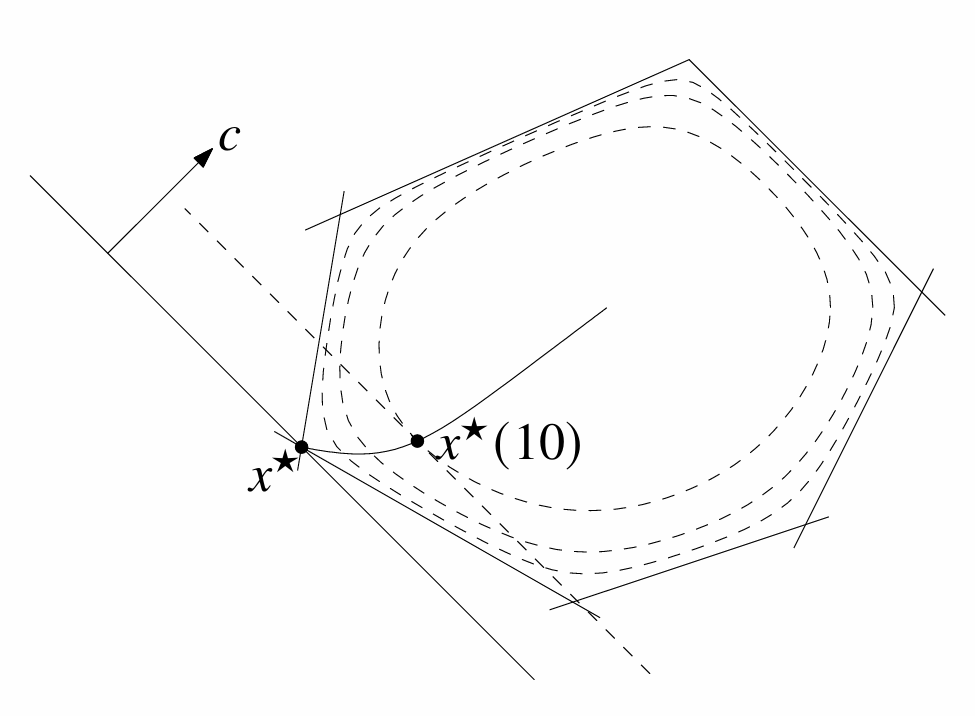
\includegraphics[width=0.75\linewidth]{img//marcoTeorico/optimizacion_fig3.png}
    \caption{Representación bidimensional del conjunto factible, el punto óptimo y la trayectoria central \( x^*(t) \) seguida por los métodos de barrera conforme el parámetro \( t \) incrementa. Se incluyen curvas de nivel que ilustran la función de barrera o, alternativamente, la función objetivo. Adaptada de~\cite[p.~361]{BoydVandenbergheSlides2023}}%
    \label{fig:optimization3}
\end{figure}

Esta contención es a menudo explotada en la práctica algorítmica. Por ejemplo, muchos métodos eficientes para resolver
problemas de optimización con restricciones de desigualdad, como los \textbf{métodos de barrera} (una clase importante
de \textbf{métodos de punto interior}\footnote{\textbf{Métodos de punto interior (\textit{Interior-point methods}):}
Una clase de algoritmos para resolver problemas de optimización lineal y no lineal convexa. A diferencia de los métodos
como el simplex que se mueven a lo largo de los bordes del conjunto factible, los métodos de punto interior generan una
secuencia de puntos estrictamente factibles en el \textit{interior} de la región factible que convergen al óptimo. A menudo
siguen una ``trayectoria central'' teórica, que es el conjunto de soluciones a una familia parametrizada de problemas de
optimización que incorporan una función de barrera (típicamente logarítmica) para las restricciones de desigualdad~\cite[Cap.~11]{BoydVandenberghe2004},~\cite[Cap.~9 y 11]{BoydVandenbergheSlides2023}.}), requieren un punto inicial
estrictamente factible (un punto $x$ tal que $f_i(x) < 0$ para todas las restricciones de desigualdad)~\cite[pp.~561, 568]{BoydVandenberghe2004},~\cite[pp.~355, 367]{BoydVandenbergheSlides2023}.

Si tal punto no se conoce de antemano, se emplea comúnmente un procedimiento de dos fases. La \textbf{fase I} consiste
en formular y resolver un problema de optimización auxiliar cuyo objetivo principal es encontrar un punto estrictamente
factible para el problema original. Si la fase I tiene éxito (es decir, encuentra un punto estrictamente factible), su
solución se utiliza como punto de partida para la \textbf{fase II}, que consiste en resolver el problema de optimización
original~\cite[p.~579]{BoydVandenberghe2004},~\cite[p.~372]{BoydVandenbergheSlides2023}. Una formulación común del
problema de fase I implica introducir una variable artificial $s$ y minimizar $s$ sujeto a las restricciones originales
modificadas, como $f_i(x) \leq s$. Este problema de fase I es en sí mismo un problema de optimización (a menudo convexo
si el original lo es) que busca determinar la factibilidad del problema original y encontrar un punto factible si existe~\cite[p.~579]{BoydVandenberghe2004},~\cite[p.~373]{BoydVandenbergheSlides2023}.\ \textit{[Aquí podría insertarse una
figura conceptual del método de barrera y la trayectoria central, como la Figura 11.2 de~\cite[p.~565]{BoydVandenberghe2004}
o la Figura 9.1 de~\cite[p.~361]{BoydVandenbergheSlides2023}, para ilustrar cómo, una vez asegurada la factibilidad
(a través de la fase I o por conocimiento previo), el algoritmo procede hacia la optimalidad manteniéndose dentro de la
región factible.]}

En resumen, la determinación de la factibilidad es un prerrequisito lógico y a menudo algorítmico para la optimización.
Un problema de optimización busca el ``mejor'' punto dentro del conjunto factible, mientras que un problema de factibilidad
simplemente busca determinar si dicho conjunto no está vacío y, en caso afirmativo, encontrar cualquier punto en él.
La capacidad de enmarcar problemas de factibilidad como problemas de optimización (con una función objetivo constante)
permite aplicar el amplio espectro de teorías y herramientas algorítmicas desarrolladas para la optimización también a la
resolución de problemas de factibilidad.